\documentclass{book}
 
%Russian-specific packages
%--------------------------------------
\usepackage[T2A]{fontenc}
\usepackage[utf8]{inputenc}
\usepackage[russian,english]{babel}
\usepackage{amsmath}
\usepackage{amssymb}
\usepackage{natbib}
%--------------------------------------
 
%Hyphenation rules
%--------------------------------------
%\usepackage{hyphenat}https://www.overleaf.com/project/5ef97fb2c79eda000172460d
%\hyphenation{ма-те-ма-ти-ка вос-ста-нав-ли-вать доп-пель-ган-гер гене-тика обще-научном}
%--------------------------------------
 
\usepackage{graphicx}
\begin{document}
\selectlanguage{russian}
%\tableofcontents

\chapter[Что такое не везёт: p-values]{Что такое не везёт и как это рассчитывать: p-values}

\section*{Cтатистическая значимость}

Словосочетание <<статистическая значимость>> (или его психологического доппельгангера, <<достоверность>>), наверное, слышали все. Медицина, генетика, опросы про зубную пасту и против зубной пасты - весь этот поток информации без статистики и без сравнения гипотез (вот для чего нужна значимость) превращается в хаос разнообразных наборов данных.

Слово <<статистика>> имеет несколько значений. К более техническому, важному для нас, мы вернёмся позже, а сейчас поговорим немного об общенаучном. Статистика и теория вероятности - это связанные способы исследования закономерностей мира. Теория вероятностей предсказывает события, исходя из моделей, и так пытается понять то, что мы видим вокруг. Монетка, игральная кость, нормальное распределение - всё это модели случайных переменных, а исходы этих переменных - это те события, которые мы можем увидеть - орёл, четыре, червяк длиной 4 сантиметра. Статистика же делает для теории вероятности черновую, обратную работу. По наблюдениям оцениваются параметры модели (об этом мы много говорили об этом в предыдущей главе), и проверяются гипотезы о пригодности модели для описания наблюдений. 

\section*{Сравнение гипотез}

Если мы одновременно думали о нескольких гипотезах (их может быть сколько угодно, но двух взаимоисключающих гипотез $\text{В} \equiv \text{!A}$ достаточно, чтоб понять, что происходит), и мы только что провели новое наблюдение  (поставили опыт, взломали сайт, посчитали попугаев), то наше доверие к каждой из этих гипотез претерпело некоторые изменения от столкновения с реальностью, представленной результатом наблюдения.  

\begin{align}\label{hyp_compare_bayes_A}
   &P\left(\text{A|obs}\right)=
   \frac{P\left(\text{obs|A}\right) P\left(\text{A}\right)}{P\left(\text{obs}\right)} = \nonumber \\
   &=\frac{P\left(\text{obs|A}\right) P\left(\text{A}\right)}{P\left(\text{obs|A}\right) P\left(\text{A}\right)+P\left(\text{obs|B}\right) P\left(\text{B}\right)} 
\end{align}

\begin{align}\label{hyp_compare_bayes_B}
   &P\left(\text{B|obs}\right)=
   \frac{P\left(\text{obs|B}\right) P\left(\text{B}\right)}{P\left(\text{obs}\right)} = \nonumber \\
   &=\frac{P\left(\text{obs|B}\right) P\left(\text{B}\right)}{P\left(\text{obs|A}\right) P\left(\text{A}\right)+P\left(\text{obs|B}\right) P\left(\text{B}\right)}
\end{align}


$P\left(\text{A|obs}\right)$ -- вероятность того, что $\text{A}$ верна, при условии того (то есть после того), что получен результат наблюдения $\text{obs}$; $P\left(\text{A}\right)$ - это априорная (до наблюдения) вероятность того, что $\text{A}$ верна, $P\left(\text{obs|A}\right)$ - условная вероятность (правдоподобие) получить результат $\text{obs}$, если $\text{A}$ верна.

Одинаковый знаменатель в формулах \eqref{hyp_compare_bayes_A} и \eqref{hyp_compare_bayes_B} -- это вероятность наблюдения $P\left(\text{obs}\right)$ (в англоязычной литературе она называется evidence). Часто при сравнении гипотез её вообще опускают, и из \eqref{hyp_compare_bayes_A} и \eqref{hyp_compare_bayes_B} получается:
\begin{align}\label{hyp_compare_bayes_comp}
   &\frac{P\left(\text{A|obs}\right)}{P\left(\text{B|obs}\right)}=\frac{P\left(\text{obs|A}\right) P\left(\text{A}\right)}{P\left(\text{obs|B}\right) P\left(\text{B}\right)}
\end{align}.

Или просто пишут 
\begin{align}\label{hyp_compare_bayes_null_prop}
   &P\left(\text{A|obs}\right)\propto P\left(\text{obs|A}\right) P\left(\text{A}\right)
\end{align}

 Значение evidence несёт важную информацию о наборе моделей (гипотез), или иными словами, о предположениях, в которых мы их сравниваем \citep[подробнее см.][]{skilling_nested_2006}. В каждом байесовском выражении у всех вероятностей справа после $\text{|}$ мы можем написать длинную цепочку условий, при которых это выражение имеет смысл. Тут будет такие предположения, как наблюдаемость мира, работоспособность приборов, правильность постановки эксперимента. Для \eqref{hyp_compare_bayes_A} - \eqref{hyp_compare_bayes_B} это ещё и предположение, что верна одна и только одна из гипотез. Обычно мы все эти условия не пишем, как очевидные, но иногда, когда модели вложены или параметризованы, явная запись части условий необходима для того, чтобы формулы заработали. 
 
 Пусть у модели $A$ есть параметр $\alpha$. Считаем его апостериорное распределение после наблюдения $\text{obs}$. Запись этого распределение имеет смысл, только если $\text{A}$ верна,
\begin{align}\label{hyp_compare_evid_A}
   P\left(\alpha\text{|obs,A}\right)=\frac{P\left(\text{obs|}\alpha\text{,A}\right) P\left(\alpha\text{|A}\right)}{P\left(\text{obs|A}\right)}
\end{align}
$P\left(\text{obs|A}\right)$ - это evidence в \eqref{hyp_compare_evid_A}, он считается как статистическая сумма по всем возможным значениям $\alpha$ - и эта же условная вероятность - $P\left(\text{obs|A}\right)$ - это значение правдоподобия гипотезы $A$ в \eqref{hyp_compare_bayes_A}. Получается, что когда мы оцениваем апостериорные распределения параметра при условии, что сама гипотеза верна, evidence -- это оценка адекватности гипотезы (модели) наблюдениям. 

\section*{Нулевые и альтернативные гипотезы}

Семейство моделей, о которых мы говорим (вернее, с пониманием молчим), когда заходит речь о статистической значимости или о p-value -- это модели, соответствующие нулевой гипотезе (Null Hypothesis). Конкретное содержание нулевой гипотезы зависит от контекста наблюдения, но общий смысл всегда один и тот же - всё плохо. Эта оптимистичная мысль объединяет собой все нулевые гипотезы. Лекарство работает так же, как плацебо, преступность не отличается между двумя городами, ген одинаково экспрессируется в разных условия, носители разных аллелей одного локуса одинаково часто болеют чем попало -- всё это примеры нулевых гипотез. 

Если нулевая гипотеза верна, то в эксперименте, мы, конечно, всё равно не увидим идеального сходства условий, идеального совпадения экспрессии генов в разных группах и прочих идеальных вариантов выполнения предположения нулевой гипотезы -- мы получим результат, порождённый шумом. Если же нулевая гипотеза не верна, то мы будем наблюдать некий содержательный сигнал, опять-таки искажённый шумом. Для того, чтобы на основании наблюдения (наблюдений), понять, насколько близка к истине нулевая гипотеза $\text{NULL}$ по сравнению с альтернативной (ненулевой) $\text{!NULL}$, можно использовать формулы условной вероятности \eqref{hyp_compare_bayes_A} - \eqref{hyp_compare_bayes_B}. 

\begin{align}\label{hyp_compare_bayes_null}
   &P\left(\text{NULL|obs}\right)=
   \frac{P\left(\text{obs|NULL}\right) P\left(\text{NULL}\right)}{P\left(\text{obs}\right)} = \nonumber \\
   &=\frac{P\left(\text{obs|NULL}\right) P\left(\text{NULL}\right)}{P\left(\text{obs|NULL}\right) P\left(\text{NULL}\right)+P\left(\text{obs|!NULL}\right) P\left(\text{!NULL}\right)} 
\end{align}

\section*{P-value}
На самом деле, \eqref{hyp_compare_bayes_null} использует редко: для этого нужно уметь оценивать распределение экспериментальных результатов не только для нулевой гипотезы, но и для альтернативной, а это требует, как минимум, построения модели содержательного сигнала. Для того, чтобы можно было сказать хоть что-нибудь о состоятельности нулевой гипотезы, не зная ничего про альтернативные, используют оценку, в чём-то родственную Байесовской (об этом ниже), но сильно упрощённую. Поскольку сравнивать нулевую гипотезу с альтернативными мы не можем, то единственная мера адекватности нулевой гипотезы наблюдениям - это вероятность наблюдений при условии того, что нуль-гипотеза верна. Её априорную вероятность при этом вообще не учитывают, как в анекдоте о том, что вероятность того, что за углом стоит тигр, равна $1/2$ - действительно, он же там или стоит, или нет. 
Следующая трудность связана с тем, что вероятность одного значения непрерывной случайной величины - это бесконечно малая величина. Она имеет смысл либо если нам нужно отношение таких вероятностей при разных предположениях, либо если мы интегрируем её на каком-то интервале. Пока в баейсовской формуле мы считали отношения, всё было в порядке, теперь надо задуматься от интервалах.

Самый понятный интервал - это от столба и до обеда. Его и используют при оценке p-value. p-value, по определению, это вероятность наблюдать тот результат, который был получен, или более маргинальный результат, при условии того, что нулевая гипотеза верна.


\begin{figure}
    \centering
    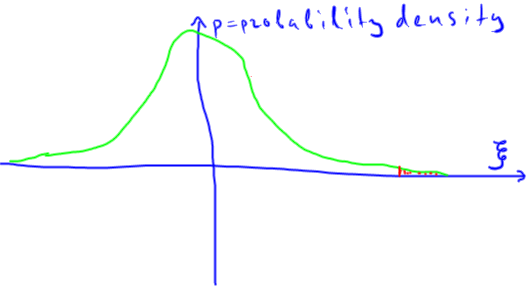
\includegraphics[scale=.5]{img/p-value.png}
    \caption{Площадь красного сегмента графика плотности вероятности случайной величины $\xi$ - это p-value, соответствующее значению $\xi$ на границе сегмента}
    \label{pval}
\end{figure}

\bibliographystyle{apalike}
\bibliography{p-values}

\end{document}
